\documentclass{article}
\usepackage{graphicx}
\usepackage[margin=1.5cm]{geometry}
\usepackage{csquotes}

\begin{document}

\title{Thursday Reading Assessment: Chapters 24-26 of \textit{Last Place on Earth}, Part II of Horizons}
\author{Prof. Jordan C. Hanson}

\maketitle

\section{Chapter 24 - The Pole Seeker Prepares}

\begin{enumerate}
\item Robert Falcon Scott ordered the \textit{Terra Nova} back to New Zealand for the winter after operations concluded in the summer.  After barely making it out of the pack ice, and the ocean freezing solid behind them, the ship made it to Lyttlelton, New Zealand.  There was a problem with the bilge pump, though, which nearly cost them the ship.  Why was it dangerous to have just one working pump?  What did Davies do to fix it?  (\textit{This type of situation is known as a single point of failure, or single POF}). \\ \vspace{2cm}
\item At ``Framheim'' Roald Amundsen and company establish a winter routine to enable good working morale through the long dark winter.  Describe some of the things they did to pass the time.  On what projects did they work?  \textbf{One example to get you started}: Roald Amundsen had the foresight to buy hickory wood from Pensacola \textit{a decade} prior to the expedition, to be used by Bjaaland for sledge-making.\\ \vspace{2cm}
\item What did the men at Framheim do with the navigational tables to avoid the single POF that occurred on Scott's prior expedition, when the only set of tables was lost just before the journey South? \\ \vspace{1cm}
\item How did the dogs help clean out the ``W.C'' (a euphemism for the toilet area) at Framheim? \\ \vspace{1cm}
\end{enumerate}

\section{Chapter 25 - Wintering at Cape Evans}

\begin{enumerate}
\item Robert Falcon Scott proposed leaving for the South Pole on November 3rd and taking 144 days to travel 1530 miles.  a) How many miles per day is this?  b) Based on what you know from prior units, does this seem reasonable if dogs are pulling the loads?  c) What methods did Scott choose to haul the gear, over the use of motor sledges and dogs? \\ \vspace{2cm}
\item One quality of leadership that was required of each captain was the ability to handle \textit{isolation.}  The author discusses how each leader deals with the paradox of being the person ``in charge,'' and therefore separate from the others, while at the same time being in close contact with the others all winter.  Compare and contrast the styles of Scott and Amundsen on this account.  \\ \vspace{2cm}
\end{enumerate}

\section{Chapter 26 - False Start}
\begin{enumerate}
\item In the days leading up to the official start of the journey to the Pole, Amundsen and his men kept pushing back the start date.  What was causing them to wait?  What was the effect on their nerves?  What finally lead to their clearange for departure? \\ \vspace{2cm}
\item Amundsen's party, with 86 dogs and 8 men, finally raced for the Pole.  Then, ``the cold counter-attacked.''  What happened next?  (Hint: everything was not \textit{opplagt}, in Norwegian.  Literally, not ``clear''). \\ \vspace{2cm}
\item The author describes the final start of Amundsen and company for the Pole with words like ``a marriage of civilization and primitive culture,'' and that ``it was to end the era of terrestrial exploration that began with the explosion of the human spirit during the Renaissance.''  Why does the author frame the adventure this way?  Do you agree with this characterization?  Why or why not?  \\ \vspace{2cm}
\end{enumerate}

\section{Horizons - Part II}

\begin{enumerate}
\item 
\begin{figure}[hb]
\centering
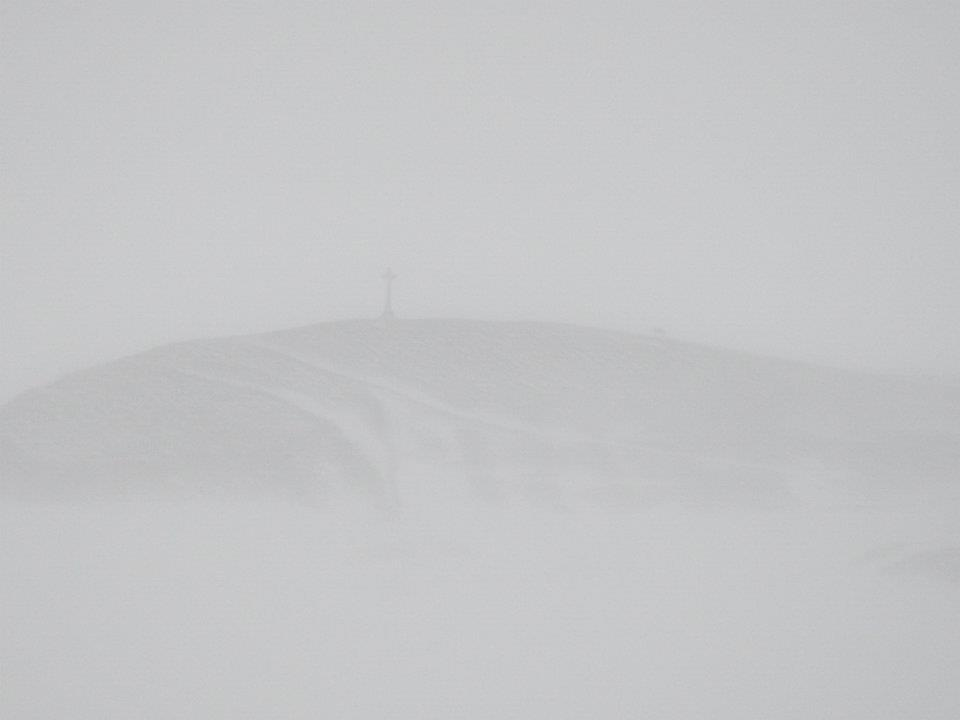
\includegraphics[width=0.35\textwidth]{cross1.jpg}
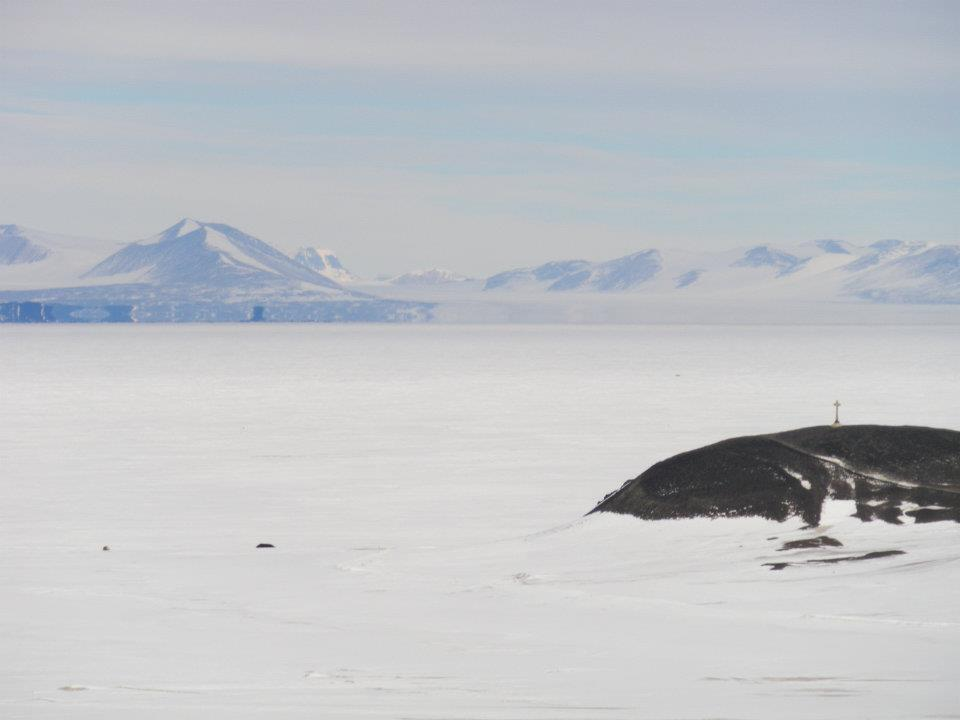
\includegraphics[width=0.35\textwidth]{cross2.jpg}
\caption{\label{fig:cross} The cross dedicated to the memory of Scott's fateful journey back from the South Pole.}
\end{figure}
(\textbf{Extra credit}).  	On page 471 of Horizons, Barry Lopez compares his perspective to that of Roland Huntford (the author of \textit{Last Place on Earth} regarding the differences between the Amundsen and Scott expeditions.  He makes reference to the cross dedicated to Scott near McMurdo (see my photos in Fig. \ref{fig:cross}).  In your opinion, how does his perspective differ from Huntford's? \\ \vspace{2cm}
\item On page 488, the author relates a story about a helicopter pilot who gives the scientists a hiding: ``The helicopter pilot, clearly irritated by something not apparent to us, began shouting at his passengers...I'd felt this tension aboard the \textit{Palmer} for some weeks, disgruntled crewmen resenting the condescending treatment they had to endure from a few of the scientists, people who strolled the ship with the air of owners.  This theme, the tension between two social classes, is the infrequently reported story, in my experience, of numerous fractious scientific and adventuring expeditions.''  How does this tension manifest itself in our community today?  How did it manifest itself on the Scott expedition?  \textit{Reflect} on how this tension has appeared in your life. \\ \vspace{4cm}
\item (\textbf{Extra credit}) As part of this essay, the author retells briefly the story of Ernest Shackleton and the \textit{Endurance} expedition.  This venture was an amazing survival story.  Can you recall what happened?  We will revisit this later! \\ \vspace{2cm}
\item How does the author view the relationship between Western civilization and the indigenous cultures located in the southern top of Latin America?  As a start you may describe the author's interactions with the native Y\'{a}mana people.  As a clue, the author also references Charles Darwin and Jean Raspail.
\end{enumerate}

\end{document}
